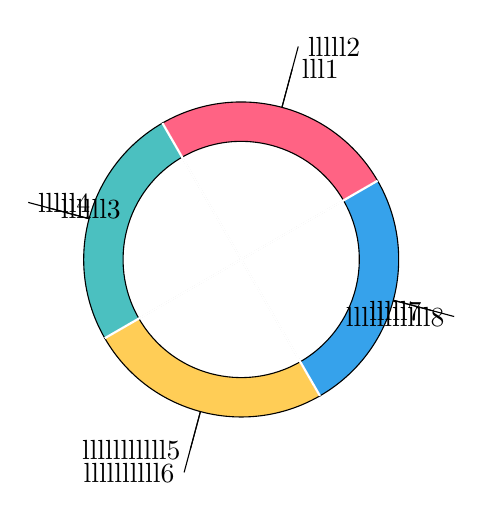
\begin{tikzpicture}
\def\innerradius{1.5cm}
\def\outerradius{2cm}
\def\gap{0.2cm}

\coordinate (o) at (0,0);

% 定义颜色
\definecolor{color1}{RGB}{255,99,132}
\definecolor{color2}{RGB}{75,192,192}
\definecolor{color3}{RGB}{255,205,86}
\definecolor{color4}{RGB}{54,162,235}

% 绘制分离的饼图块
\draw[fill=color1] (o) -- (30:\outerradius) arc (30:120:\outerradius) -- (120:\innerradius) arc (120:30:\innerradius) -- cycle;
\draw[fill=color2] (o) -- (120:\outerradius) arc (120:210:\outerradius) -- (210:\innerradius) arc (210:120:\innerradius) -- cycle;
\draw[fill=color3] (o) -- (210:\outerradius) arc (210:300:\outerradius) -- (300:\innerradius) arc (300:210:\innerradius) -- cycle;
\draw[fill=color4] (o) -- (300:\outerradius) arc (300:390:\outerradius) -- (390:\innerradius) arc (390:300:\innerradius) -- cycle;

% 绘制分割线
\foreach \x in {30,120,210,300}{
  \draw[thick,white] (o) -- (\x:\outerradius);
}

% 绘制标签和折线
\draw (75:\outerradius) -- +(75:0.5) node[anchor=west] {lll1};
\draw (75:\outerradius) -- +(75:0.8) node[anchor=west] {lllll2};

\draw (165:\outerradius) -- +(165:0.5) node[anchor=west] {llllll3};
\draw (165:\outerradius) -- +(165:0.8) node[anchor=west] {lllll4};

\draw (255:\outerradius) -- +(255:0.5) node[anchor=east] {lllllllllll5};
\draw (255:\outerradius) -- +(255:0.8) node[anchor=east] {llllllllll6};

\draw (345:\outerradius) -- +(345:0.5) node[anchor=east] {lllll7};
\draw (345:\outerradius) -- +(345:0.8) node[anchor=east] {lllllllllll8};

\end{tikzpicture}